\chapter{Event Simulation}
\label{sim}
%somewhere have the pretty picture from 
%matt mc tutorial on how generators/geant/etc 
%fit in with everything else (reco, whatever)

%ARXIV PAPER OF AWESOMENESS
%http://arxiv.org/abs/hep-ph/0403045

%PYTHIA MANUAL OF AWESOMENESS
% the one I'm looking at is lutp0613man2.pdf, 
% but there's probably a more recent one




% I THINK I HAVE TOO MANY LONG SENTENCES 
% AND PREPOSITIONAL PHRASES


%need for event simulation: 

Within %the role of % CHANGE THIS CONSTRUCTION
a high-energy physics experiment's role of making 
discoveries and measurements, 
it necessary to know ahead of time what exactly 
should be expected. 
What will the detector signature of a new process look like? 
How will we know whether we've seen something unexpected? 
This is where event simulation contributes.  
%what exactly is the simulated data
Essentially, a series of programs is used to carefully 
generate and calculate all the relevant quantities for a set of 
fake events.  
This information is then used 
to aid analysis in ways for which 
real data alone cannot suffice.  

Having the ability to simulate physics processes 
serves multiple purposes. 
It aids in detector design: 
knowing the expected typical characteristics of particle 
interactions is essential to design a detector 
suited for those interactions.  
Once the detector design is settled, 
simulation of the detector is useful to design 
the algorithms used to reconstruct particles 
from their signature interactions with the 
detector material.  
In addition, simulating the physics processes 
can give estimates of how many 
events of a particular type are expected, 
further aiding the design process.  
The event simulation also contributes 
directly to many analyses, 
in the way of calculating the acceptance, 
the fraction of events that can theoretically 
be detected (see Section~\ref{FIXME}): 
it is impossible to know from observation 
how many events are missed by the detector, 
because of the very fact that they are unseen.  
It is instead necessary to get that fraction 
from a framework in which 
the characteristics of all events are 
inherently known, not reconstructed.  
Finally, % and possibly most visibly (?) I don't like that
simulated data is directly compared 
with ``real'' data from the detector 
to interpret the real-data results.  
If the data shows something significantly 
different from the simulation, 
then something is missing: 
perhaps a calibration needs to be applied, 
or the response of a detector unit needs 
to be further understood.  
Or, perhaps, there is a new physics process 
appearing for the first time, 
which was not previously known and 
which was therefore not present in the simulation.  
In this case simulation of proposed new physics 
processes may narrow down the identity of the 
observed new process.  
Whatever the case, 
discrepancy between observed data and the event 
simulation indicates that further 
investigation is necessary.  


%points of event simulation: 

%   * directly relevant: compare with data (description of current understanding as is) 
%-- we want to be able to interpret what we're seeing 
%in terms of what physics process it might be

%   * also relevant: acceptance is necessarily a MC calculation!

%   * also: design detectors, design reconstruction and other (e.g. trigger) algorithms

%   * also: event rates (like trigger rates?)  

The entire detection process is simulated, 
including the protons' direct interaction 
and any subsequent particle decays, 
as well as how the end-product particles 
interact with the detector as they pass through 
and how the detector itself responds.  
This latter part includes not only the 
material of the individual subdetectors 
but also the algorithms of 
the Level-1 Trigger, 
which are implemented in hardware 
(see Section~\ref{exp:L1}).  
The High-Level Trigger does not need to be 
simulated in this way; 
since its algorithms are all software-based, 
the same code can be run without modification 
on both real data and simulated data.  



\section{Monte Carlo Event Generation}
\label{sim:MC}
put why called ``monte carlo'', 
also connect ``event simulation'' terminology 
with ``generator'' and the multiple types thereof.
like, ``simulation'' broken down into several steps, 
one of which is the generation of the main 
physics process itself (aka ``hard physics process'')
HOW the events are actually ``generated'', 
like the whole random number business. 
It uses a random number generator , 
to determine ``in a probabilistic way'' -- 
only one main interaction happens 
for each proton (bunch) interaction, 
but the sum over all events ,
according to the probability of each type of 
interaction happening.  



\subsection{Put this stuff in its own section?}
\label{sim:MCexplain}

%types of programs with different types of output -- what they're used for. 
%start with tree-level stuff and dsigma eqn...

%   * cross section integrators

%   * event generators

There are two sorts of programs that can be called 
%``Monte Carlo generators''.  
``Monte Carlo event simulators''.  
They both use the matrix elements derived from 
the Feynman diagrams of the physics interactions of interest 
(explained in Section~\ref{FIXME}), % THAT MEANS EXPLAIN ALL THIS STUFF IN PREVIOUS CHAPTER
but they use the matrix element formalism 
in different ways to achieve different ends.  
As a reminder, the equation to obtain the 
differential cross section % WHAT'S IT ACTUALLY CALLED??
from the matrix element for a given diagram is 

\[
d\sigma = \frac{1}{\hat{s}}|\mathcal{M}|^2 \frac{d \cos \theta d\phi}{8(2\pi)^2}
\]

The first type of Monte Carlo program outputs 
a single quantity or set of quantities characteristic 
of the given process, 
such as the cross section.  
These programs are called ``cross section integrators''.  
They calculate 
$d\sigma$ for each of a uniform distribution of 
phase space vales (i.e. uniform increments 
of $\cos\theta$ and $\phi$).  
$d\sigma$ represents each event's ``weight''; 
the total cross section $\sigma$ is then obtained 
by integrating over the full collection of $d\sigma$ values.  
The final result is a value for the cross section; 
hence the name.  
However, since the events themselves are distributed 
uniformly in $\cos\theta$ and $\phi$, 
their characteristics 
do not represent actual event distributions 
(real event distributions in data have 
non-uniform distributions, 
in $\cos\theta$ in particular).  
Therefore they can only be used to calculate 
a few select quantities; 
they can't be used to predict distributions.  

The second type of program are called ``event generators''.  
They also use the matrix element to calculate 
the differential cross section % REAL NAME
with the equation given above.  
However, instead of using $d\sigma$ as an event weight, 
it ``unweights'' the events to obtain the physical 
distributions.  
It does this through the so-called acceptance-rejection method: 
first the maximum possible value of $d\sigma$ is calculated, 
$d\sigma_{max}$. 
Each event's individual $d\sigma$ value, 
the ratio $\frac{d\sigma}{d\sigma_{max}}$ is taken; 
this number is necessarily a fraction between 0 and 1.  
A random number $g$ between 0 and 1 is then generated.  
If the ratio $\frac{d\sigma}{d\sigma_{max}}$ is greater 
than $g$, then then event is kept.  
Otherwise, it is rejected.  
This method causes the generated events to have the properties 
and distributions that events would have in reality -- 
sections of phase space with a higher ``event weight'' 
are more likely to be represented.  

%tree-level all well and good, but need corrections to really 
%make things realistic.  
%ways of doing the corrections:

%   * matrix element

%   * parton shower

However, using a single Feynman diagram is not typically 
sufficient to make very accurate calculations.  
%a number or determine distributions is not typically 
%sufficient.  
In general, there are significant contributions from 
the higher-order diagrams  
(diagrams with more legs and loops, 
but still representing the same final arrangement of particles). 
These corrections must be taken into account.  
In addition, the matrix elements and Feynman diagrams 
for these calculations only consider bare quarks, 
that is, quarks extracted from the framework of 
hadrons such as the proton.  
These bare quarks cannot exist in reality, 
so a method of accounting for the quarks 
as being inside hadrons must also be used.  
There have been two different paths taken to deal % path = tack? track?...
with the above issues.  
In the first, the ``matrix element'' method, 
Higher-order diagrams are explicity included in 
the matrix element calculation.  
Since the higher the order, 
the more complex the calculation, 
only diagrams of up to a given order are 
generally used.  
In one implementation, more ``legs'' can be dealt with, 
but diagrams containing virtual loops are ignored.  % EXPLAIN IN PREVIOUS CH
In the other, all diagrams, including those with virtual 
loops, of a single order are used, 
but at the moment there exist satisfactory solutions 
only for next-to-leading-order diagrams 
(or NLO, explained in Section~\ref{FIXME}).  
%only for diagrams one step higher 
%than the basic tree-level diagram
The matrix element method does not explicitly 
take care of the bare-quark problem; %, though.  
this can be handled in multiple ways.  
%Programs who do not deal with the interactions of 
Some cross section integrators deal with the interactions of % is it only cross section integrators??
quarks inside hadrons using Feyman's factorization theorem. 
Programs which do not deal with them in this way 
can be interfaced with programs following the 
second of the two paths, %.  
%The second path is called 
the ``parton shower'' method, 
which is the method used by many event generators 
(as opposed to cross section integrators).  
In the parton shower method, 
instead of including diagrams representing 
higher orders and quarks-within-hadrons 
into the matrix element calculation, 
this part of the interaction is taken care of 
by a separate routine.  
This routine takes the products of the 
basic tree-level interaction 
and decays them according to 
probabilities and rules coded into the program.  
The process is iterative, 
repeating for any quarks or gluons that 
branch off at any point.  
In this way the parton shower method 
is more flexible than the matrix element method -- 
it can deal with many branchings and legs. 
However, it is also less precise formally, 
since it avoids the use of the matrix elements 
from the Feynman diagrams.  

%where do the PDFs fit in?  just to parton shower method?? 
%no, it looks like PDFs have to enter in both 
%ways of doing hadronization. 
%(actually, is it only just the initial 
%proton interaction where you need the PDFs?? 
%inside a proton is the only place 
%where x is a relevant quantity...
%dunno, skirt for now)

%do I need more detail at this point?  
%I guess still need to explain modular structure... 
%can more specific stuff like hadronization 
%model go just under pythia, or should it 
%go here?  
%I guess should be more general, 
%since those algorithms are more general.  
%SO, HERE

The philosophy of parton-shower generators 
in particular 
is that the entire process of simulating 
a physics event can be done in a modular fashion.  
Fig.~\ref{fig:MCsteps} 
shows the typical steps necessary to simulate an events.  
The incoming protons are modeled in terms of the 
parton distribution functions (Section~\ref{FIXME}).  % NEED TO EXPLAIN ``PARTONS'' IN THAT SECTION
The ``hard subprocess'' refers to the main 
physics interaction.  
Not shown in the diagram are other interactions 
involving different parts of the protons 
or other protons in the same bunch; 
these interactions are not as interesting 
because they are typically not as energetic.  
The participant particles in the main interaction 
are then ``evolved'' through the showering process, 
which includes emissions of photons or gluons 
by the initial or final particles, 
as well as ``branchings'' of final particles. % INCLUDED IN FORMER?? 
Any resulting quarks and gluons are 
formed into ``colorless'' hadrons, 
which may then decay into other particles. 
These final particles are the ones seen 
in the detector.  
The fact that the full process can be separated 
into these steps 
makes it easier for different programs 
to handle individual steps.  
For example, one program may simulate the 
hard process, 
while another is better-equipped to take care 
of the showering and hadronization, 
and a third is specialized in the decay of 
a particular particle.  
To further the theme of modularity, 
the fully-decayed situation 
is then plugged into a program simulating 
the passage of the particles through the detector 
and the detector's response (Section~\ref{FIXME}).  

%And how these two things fulfill the different needs for 
%both higher orders and hadronization

%BIG PRETTY PARTON SHOWER PICTURE but also need to explain PDF part, etc. etc. 
should compare to other one from zeus people, which one is better? 

 \begin{figure}[htb]
  \begin{center}
    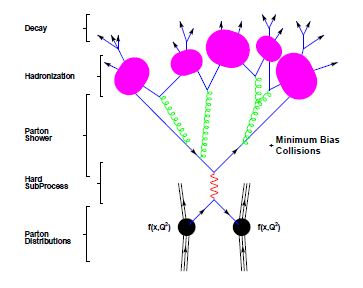
\includegraphics{Figures/mc-partonShower-lesHouches.png}
  \end{center}
  \caption[Diagram of typical steps used to simulate event in parton shower method]
	  {Diagram of typical steps used to simulate event in parton shower method.
	    The incoming protons are modeled in terms of the 
	    parton distribution functions. 
	    The ``hard subprocess'' refers to the main 
	    physics interaction.  
	    The participant particles in the main interaction 
	    are then ``evolved'' through the showering process, 
	    which includes emissions of photons or gluons 
	    by the initial or final particles, 
	    as well as ``branchings'' of final particles. % INCLUDED IN FORMER?? 
	    Any resulting quarks and gluons are 
	    formed into ``colorless'' hadrons, 
	    which may then decay into other particles. 
	    These final particles are the ones seen 
	    in the detector.  
	  }
  \label{fig:MCsteps}
 \end{figure}


and lund string model pictures (both, yay!)

 \begin{figure}[htb]
  \begin{center}
%    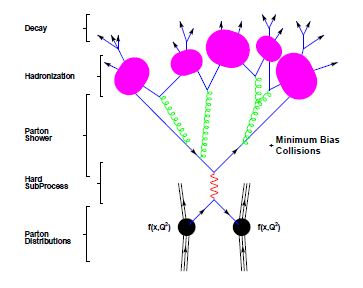
\includegraphics{Figures/mc-partonShower-lesHouches.png}
    \subfloat[]{\label{fig:MClundA}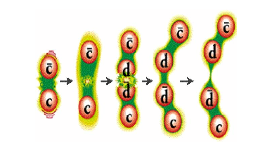
\includegraphics{Figures/mc-lundStringModel-zeusPeople.png}}
    \subfloat[]{\label{fig:MClundB}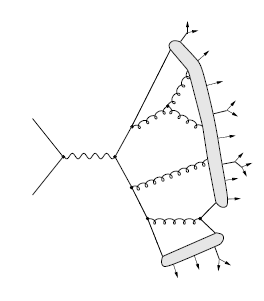
\includegraphics{Figures/mc-lundStringDiagram-zeusPeople.png}}
  \end{center}
  \caption[Schematics showing the Lund string model of hadronization]
	  {Schematics showing the Lund string model of hadronization.}
  \label{fig:MClund}
 \end{figure}



pythia is definitely parton shower, 
explain steps and hadronization model, etc

%\subsection{some explanation of the black box?}
%\label{sim:MCBlackBox}
% it's not really a black box anymore!
%can talk about black-box mentality in introduction
%modular structure here?  that pretty picture showing all the 
%different steps to an interaction that need to be 
%simulated. 
%all those steps can be done by separate packages, 
%which is the philosophy.  (pythia manual)
%pdfs ->
%hard scatter (underlying event, multiple interactions in parallel) ->
%[parton] shower (both isr and fsr, incl QED) ->
%hadronization (not directly applicable to my process, but applicable for bg's) -> 
%decay resonances -> interactions with detector material ...

\subsection{Monte Carlo Generator Programs}
\label{sim:MCGens}

short intro on programs: pythia, powheg, tauola, fewz

HOW THE PROGRAMS USED TO GENERATE THESE SAMPLES AND NUMBERS 
FIT INTO THIS FRAMEWORK.  
   pythia, powheg, tauola, fewz... else??  (didn't end up using MCatNLO) 
I don't think anything else.  
also explain about fewz different (xsec integrator, sounds like)

I feel like I remember seeing something from herwig?? in one of the 
production config fragments...

\subsubsection{PYTHIA}
\label{sim:MCGensPythia}

PYTHIA THE MONSTER

what are the different tunes for?  tune z2, tune d6t

\subsubsection{POWHEG}
\label{sim:MCGensPowheg}
why is this one used in favor of pythia?  
more to the point, what exactly is it? 
and how is it different from pythia? 

\subsubsection{Other Generators}
\label{sim:MCGensOther}
Like, whichever other samples I check (background etc) -- actually, they're all pythia

TAUOLA AND FEWZ

AND, FEWZ webpage was on frank petriello's wisconsin space and doesn't exist anymore

http://www.phys.hawaii.edu/~kirill/FEHiP.htm links to 
http://www.hep.wisc.edu/~frankjp/FEWZ.html (bad link)

FEWZ 2.0 abstract on the arXiv: http://arxiv.org/abs/1011.3540 
from ryan gavin, ye li, frank petriello, and seth quackenbush (15 Nov 2010)

WHICH VERSION DID VBTF USE??  look at syst AN.  
e-mail frank about documentation page??

https://indico.cern.ch/getFile.py/access?contribId=38\&resId=3\&materialId=slides\&confId=71330  tutorial from ryan giving original arXiv references (non-2.0)




\section{Detector Simulation}
\label{sim:Detector}
%\subsection{GEANT Detector Model/Modeling of Particle Interactions in Detector Material}

\subsection{GEANT Detector Model}
\label{sim:DetectorGeant}

GEANT the giant

\subsection{Level-1 Trigger Emulator}
\label{sim:DetectorL1Emul}
talk about how emulator necessary for l1, but not for hlt (duh)
